

\begin{frame}{Resultados e Discussão}
    Segundo \citeonline[p.~68]{morgado-geometria-i}, ``as mediatrizes dos lados de um triângulo cortam-se em um ponto denominado circuncentro, que é o centro do círculo que passa pelos três vértices''. A Figura \ref{fig:triangulo} mostra um triângulo $ABC$ inscrito em uma circunferência de centro $O$ e raio $r$.
    \vfill
    \begin{figure}[H]
        \centering
        \caption{Triângulo $ABC$ inscrito}
        \label{fig:triangulo}
        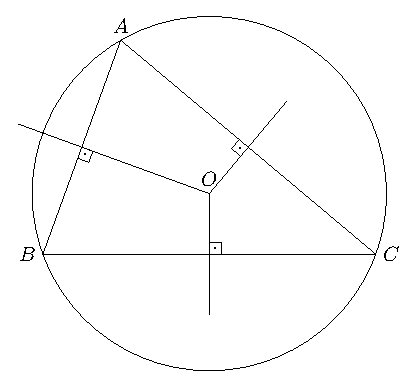
\includegraphics[width=0.3\textwidth]{img/modelo/tikz/circuncentro.pdf}\\
        \footnotesize{Fonte: \citeonline[p.~68]{morgado-geometria-i}, adaptado.}
    \end{figure}
\end{frame}


% Seção de Resultados e Discussão
\section{Resultados e Discussão}
% Slide da seção de Resultados e Discussão
\begin{frame}{Resultados e Discussão}
    \begin{block}{Teorema da Probabilidade Total \cite{morgado-combibatoria}}
        Se $B$ é um evento contido numa união de eventos disjuntos
        $$
        A_1, A_2, \cdots, A_{n}, \text{ e}
        $$
        $$
        P(A_1) > 0, P(A_2) > 0, \cdots, P(A_n) > 0,
        $$
        então,
        $$
        P(B) = P(A_1)P(B/A_1) + P(A_2)P(B/A_2) + \cdots + P(A_n)P(B/A_n).
        $$
    \end{block}
\end{frame}

% Slide da seção de Resultados e Discussão
\begin{frame}[t]{Resultados e Discussão}
\begin{block}{Parábola, conforme \citeonline{ma23-GA}}
    \begin{minipage}[t]{0.5\textwidth}
        Sejam $\mathcal{L}$ uma reta e $F$ um ponto do plano não pertencente a $\mathcal{L}$. A \textbf{parábola} $\mathcal{P}$ de \textbf{foco} $F$ e \textbf{diretriz} $\mathcal{L}$ é o conjunto de todos os pontos do plano cuja distância a $F$ é igual à sua distância a $\mathcal{L}$.
        $$
        \mathcal{P} = \{P | d(P,F) = d(P, \mathcal{L})\}
        $$
    
    \end{minipage}
    \hfill
    \begin{minipage}[t]{0.5\textwidth}
        \begin{figure}[H]
            \centering
            \caption{Parábola $\mathcal{P}: y^2 = 4px$}
            \label{fig:parabola}
            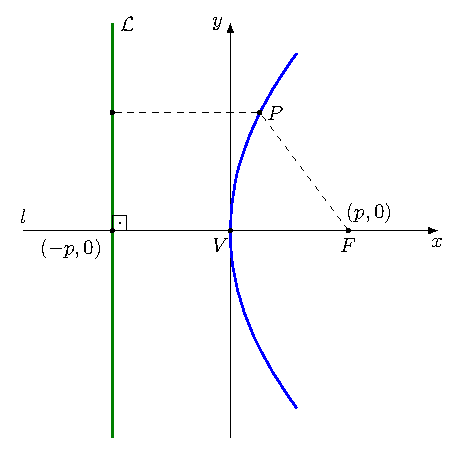
\includegraphics[width=0.6\textwidth]{img/modelo/parabola.pdf}\\
            \footnotesize{Fonte: \citeonline{ma23-GA}, adaptado.}
        \end{figure}
    \end{minipage}
\end{block}
\end{frame}

% Slide da seção de Resultados e Discussão
\begin{frame}{Resultados e Discussão}
    \begin{block}{Definição da derivada num ponto \cite{lima-analise}}
        Sejam $X \subset \mathbb{R}$, $f: X \rightarrow \mathbb{R}$ e $a \in X \cap X^\prime$ (isto é, $a$ é um ponto de acumulação de $X$ pertencente a $X$).

        Diremos que $f$ é \textit{diferenciável} no ponto $a$ quando existir o limite:

        $$
        f^{\prime}(a) = \lim_{x \rightarrow a} \dfrac{f(x)-f(a)}{x-a}.
        $$
    \end{block}
\end{frame}

% Slide da seção de Resultados e Discussão
\begin{frame}{Resultados e Discussão}
    A Tabela \ref{tab:forca} mostra fatores de conversão para unidades de força.
    \vfill
    \begin{table}[H]
        \centering
        \caption{Fatores de conversão de unidades de força}
        \label{tab:forca}
        \begin{tabular}{l l l}
            \hline 
             & N & lb\\ \hline
             1 newton & 1 & 0,2248\\ 
             1 libra & 4,448 & 1\\ \hline
        \end{tabular}
        \\
        \footnotesize{Fonte: \citeonline{serway-mecanica}}
    \end{table}
\end{frame}

% Slide da seção de Resultados e Discussão
\begin{frame}{Resultados e Discussão}
    O Quadro \ref{quadro:unidades-si} mostra as unidades base do Sistema Internacional (SI).

    \setcounter{table}{0}
    \captionsetup[table]{name=Quadro}
    \begin{table}[H]
        \centering
        \caption{Unidades do SI}
        \begin{tabular}{|l | c | c|}
             \hline
             \rowcolor{UFTgray!10}
             & \multicolumn{2}{ c|}{\textbf{Unidade base SI}} \\ \hline
             \rowcolor{UFTgray!10} \textbf{Quantidade base} & \textbf{Nome} & \textbf{Símbolo}\\
             \hline
             Comprimento & metro & m\\ \hline
             Massa & quilograma & kg\\ \hline
             Tempo & segundo & s\\ \hline
             Corrente elétrica & ampère & A\\ \hline
             Temperatura & kelvin & K\\ \hline
             Quantidade de substância & mol & mol \\ \hline
             Intensidade luminosa & candela & cd\\ \hline
        \end{tabular}
        \\
        \footnotesize{Fonte: \citeonline{serway-mecanica}}
        \label{quadro:unidades-si}
    \end{table}
\end{frame}